\documentclass[12pt]{article}
\usepackage[margin=1in]{geometry}
\usepackage{amsmath,amssymb}
\usepackage{tikz}
\usetikzlibrary{positioning, arrows.meta, shapes.geometric, fit, calc, backgrounds, decorations.pathreplacing, patterns, shadows}
\usepackage{xcolor}
\usepackage{caption}
\usepackage{float}
\usepackage{enumitem}

% Brand colors
\definecolor{Garnet}{HTML}{73000A}
\definecolor{Atlantic}{HTML}{466A9F}
\definecolor{Congaree}{HTML}{1F414D}
\definecolor{Horseshoe}{HTML}{65780B}
\definecolor{Rose}{HTML}{CC2E40}
\definecolor{Honeycomb}{HTML}{A49137}
\definecolor{Black90}{HTML}{363636}
\definecolor{Black70}{HTML}{5C5C5C}
\definecolor{Black50}{HTML}{A2A2A2}
\definecolor{Black30}{HTML}{C7C7C7}
\definecolor{Black10}{HTML}{ECECEC}
\definecolor{Sandstorm}{HTML}{FFF2E3}
\definecolor{Grass}{HTML}{CED318}

\title{\textbf{How Plug-and-Play PPO Works}\\[0.3em]
\large RL-Based Point Prompt Optimization for SAM Segmentation}
\author{Explainer for CSCE 775 Proposal 4}
\date{}

\begin{document}
\maketitle
\thispagestyle{empty}

% ============================================================
% DIAGRAM 1: THE PROBLEM — PROMPT SENSITIVITY
% ============================================================
\section*{1. The Problem: SAM Is Sensitive to Where You Click}

SAM (Segment Anything Model) can segment \textit{any} object in an image, but you have to tell it \textit{where} to look by giving it point prompts. The quality of the segmentation depends heavily on where those points are placed.

\begin{figure}[H]
\centering
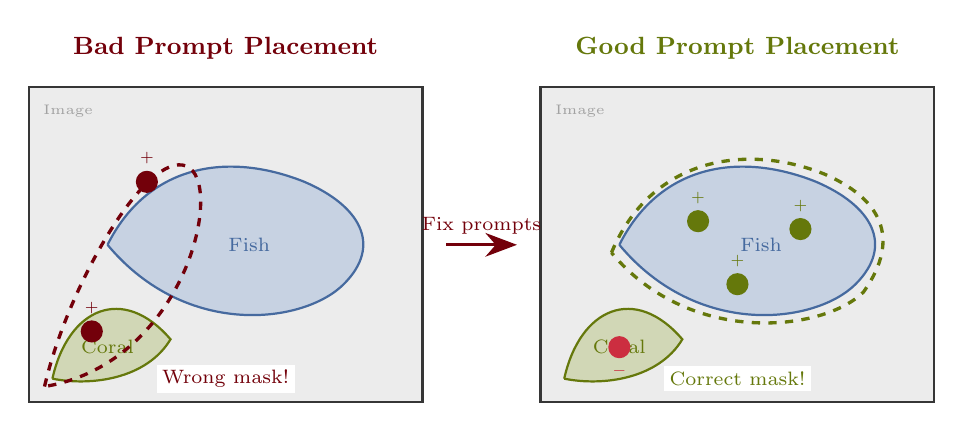
\begin{tikzpicture}[
    every node/.style={font=\small}
]

% === LEFT PANEL: Bad prompts ===
\node[font=\small\bfseries, color=Garnet] at (2.5, 4.5) {Bad Prompt Placement};

% Image background
\draw[thick, Black90, fill=Black10] (0,0) rectangle (5,4);
\node[font=\tiny, Black50] at (0.5, 3.7) {Image};

% Fish object (irregular blob)
\fill[Atlantic!30, draw=Atlantic, thick]
    (1.0, 2.0) .. controls (1.5, 3.0) and (2.5, 3.2) ..
    (3.5, 2.8) .. controls (4.2, 2.5) and (4.5, 2.0) ..
    (4.0, 1.5) .. controls (3.5, 1.0) and (2.0, 0.8) ..
    (1.0, 2.0);
\node[font=\scriptsize, Atlantic] at (2.8, 2.0) {Fish};

% Coral object
\fill[Horseshoe!30, draw=Horseshoe, thick]
    (0.3, 0.3) .. controls (0.5, 1.2) and (1.2, 1.5) ..
    (1.8, 0.8) .. controls (1.5, 0.3) and (0.8, 0.2) ..
    (0.3, 0.3);
\node[font=\scriptsize, Horseshoe] at (1.0, 0.7) {Coral};

% Bad prompt points (on wrong object / edge)
\fill[Garnet] (0.8, 0.9) circle (4pt);
\node[font=\tiny, Garnet, above] at (0.8, 1.0) {+};
\fill[Garnet] (1.5, 2.8) circle (4pt);
\node[font=\tiny, Garnet, above] at (1.5, 2.9) {+};

% Bad mask result (dashed, wrong area)
\draw[Garnet, very thick, dashed]
    (0.2, 0.2) .. controls (0.5, 1.5) and (1.5, 3.2) ..
    (2.0, 3.0) .. controls (2.5, 2.8) and (2.0, 0.5) ..
    (0.2, 0.2);

% Result label
\node[font=\scriptsize, Garnet, fill=white, inner sep=2pt] at (2.5, 0.3) {Wrong mask!};


% === RIGHT PANEL: Good prompts ===
\node[font=\small\bfseries, color=Horseshoe] at (9.0, 4.5) {Good Prompt Placement};

% Image background
\draw[thick, Black90, fill=Black10] (6.5,0) rectangle (11.5,4);
\node[font=\tiny, Black50] at (7.0, 3.7) {Image};

% Fish object (same shape)
\fill[Atlantic!30, draw=Atlantic, thick]
    (7.5, 2.0) .. controls (8.0, 3.0) and (9.0, 3.2) ..
    (10.0, 2.8) .. controls (10.7, 2.5) and (11.0, 2.0) ..
    (10.5, 1.5) .. controls (10.0, 1.0) and (8.5, 0.8) ..
    (7.5, 2.0);
\node[font=\scriptsize, Atlantic] at (9.3, 2.0) {Fish};

% Coral object
\fill[Horseshoe!30, draw=Horseshoe, thick]
    (6.8, 0.3) .. controls (7.0, 1.2) and (7.7, 1.5) ..
    (8.3, 0.8) .. controls (8.0, 0.3) and (7.3, 0.2) ..
    (6.8, 0.3);
\node[font=\scriptsize, Horseshoe] at (7.5, 0.7) {Coral};

% Good prompt points (well-placed on fish)
\fill[Horseshoe] (8.5, 2.3) circle (4pt);
\node[font=\tiny, Horseshoe, above] at (8.5, 2.4) {+};
\fill[Horseshoe] (9.8, 2.2) circle (4pt);
\node[font=\tiny, Horseshoe, above] at (9.8, 2.3) {+};
\fill[Horseshoe] (9.0, 1.5) circle (4pt);
\node[font=\tiny, Horseshoe, above] at (9.0, 1.6) {+};

% Negative point (on coral, keeping it out)
\fill[Rose] (7.5, 0.7) circle (4pt);
\node[font=\tiny, Rose, below] at (7.5, 0.6) {$-$};

% Good mask result (matches fish closely)
\draw[Horseshoe, very thick, dashed]
    (7.4, 1.9) .. controls (7.9, 3.1) and (9.1, 3.3) ..
    (10.1, 2.9) .. controls (10.8, 2.6) and (11.1, 2.1) ..
    (10.6, 1.4) .. controls (10.1, 0.9) and (8.4, 0.7) ..
    (7.4, 1.9);

% Result label
\node[font=\scriptsize, Horseshoe, fill=white, inner sep=2pt] at (9.0, 0.3) {Correct mask!};

% Arrow between panels
\draw[-{Stealth[length=4mm]}, very thick, Garnet] (5.3, 2.0) -- node[above, font=\scriptsize] {Fix prompts} (6.2, 2.0);

\end{tikzpicture}
\caption{\textbf{The core problem.} SAM needs point prompts (\textcolor{Horseshoe}{\textbf{+}} = foreground, \textcolor{Rose}{\textbf{--}} = background) to know what to segment. Badly placed prompts (left) produce wrong masks. Well-placed prompts (right) produce accurate masks. The question is: how do we \textit{automatically} find good prompt locations?}
\label{fig:problem}
\end{figure}


% ============================================================
% DIAGRAM 2: THE REFERENCE-TARGET SETUP
% ============================================================
\section*{2. Step 1: Start with a Reference Image}

The system begins with a \textit{reference image} where we already know the correct segmentation (ground truth mask). It uses this to find candidate prompt locations on a new \textit{target image}.

\begin{figure}[H]
\centering
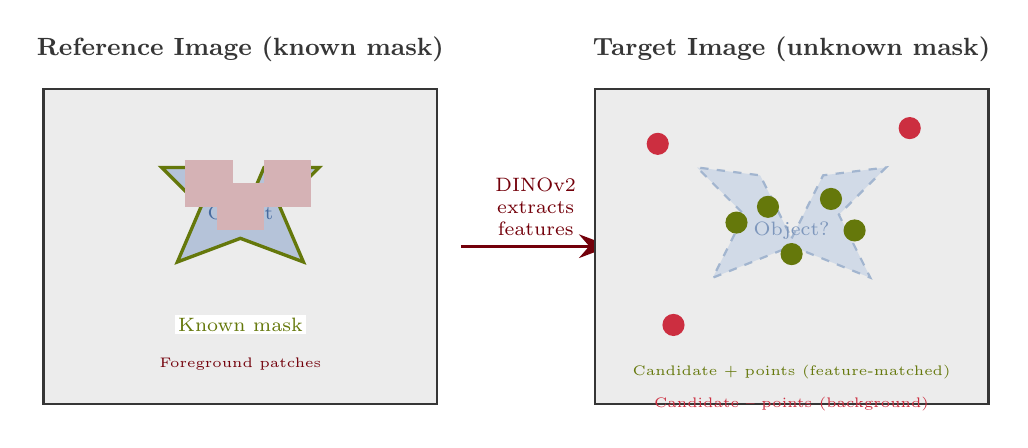
\begin{tikzpicture}[
    every node/.style={font=\small}
]

% === REFERENCE IMAGE ===
\node[font=\small\bfseries, Black90] at (2.5, 5.0) {Reference Image (known mask)};
\draw[thick, Black90, fill=Black10] (0, 0.5) rectangle (5, 4.5);

% Star-shaped object (reference)
\fill[Atlantic!40, draw=Atlantic, thick]
    (2.5, 2.8) -- (2.8, 3.5) -- (3.5, 3.5) -- (3.0, 3.0) --
    (3.3, 2.3) -- (2.5, 2.6) -- (1.7, 2.3) -- (2.0, 3.0) --
    (1.5, 3.5) -- (2.2, 3.5) -- cycle;
\node[font=\scriptsize, Atlantic] at (2.5, 2.9) {Object};

% Ground truth mask overlay
\draw[Horseshoe, very thick]
    (2.5, 2.8) -- (2.8, 3.5) -- (3.5, 3.5) -- (3.0, 3.0) --
    (3.3, 2.3) -- (2.5, 2.6) -- (1.7, 2.3) -- (2.0, 3.0) --
    (1.5, 3.5) -- (2.2, 3.5) -- cycle;
\node[font=\scriptsize, Horseshoe, fill=white, inner sep=1pt] at (2.5, 1.5) {Known mask};

% Foreground patches highlighted
\fill[Garnet!30] (2.2, 2.7) rectangle (2.8, 3.3);
\fill[Garnet!30] (1.8, 3.0) rectangle (2.4, 3.6);
\fill[Garnet!30] (2.8, 3.0) rectangle (3.4, 3.6);
\node[font=\tiny, Garnet] at (2.5, 1.0) {Foreground patches};

% === DINOv2 ARROW ===
\draw[-{Stealth[length=4mm]}, very thick, Garnet] (5.3, 2.5) -- node[above, font=\scriptsize, text width=2cm, align=center] {DINOv2\\extracts\\features} (7.2, 2.5);

% === TARGET IMAGE ===
\node[font=\small\bfseries, Black90] at (9.5, 5.0) {Target Image (unknown mask)};
\draw[thick, Black90, fill=Black10] (7.0, 0.5) rectangle (12.0, 4.5);

% Similar star-shaped object (target, slightly different)
\fill[Atlantic!25, draw=Atlantic!50, thick, dashed]
    (9.5, 2.6) -- (9.9, 3.4) -- (10.7, 3.5) -- (10.1, 2.9) --
    (10.5, 2.1) -- (9.5, 2.5) -- (8.5, 2.1) -- (8.9, 2.9) --
    (8.3, 3.5) -- (9.1, 3.4) -- cycle;
\node[font=\scriptsize, Atlantic!70] at (9.5, 2.7) {Object?};

% Candidate prompt points from feature matching
\fill[Horseshoe] (9.2, 3.0) circle (4pt);
\fill[Horseshoe] (10.0, 3.1) circle (4pt);
\fill[Horseshoe] (9.5, 2.4) circle (4pt);
\fill[Horseshoe] (8.8, 2.8) circle (4pt);
\fill[Horseshoe] (10.3, 2.7) circle (4pt);

% Negative candidates
\fill[Rose] (8.0, 1.5) circle (4pt);
\fill[Rose] (11.0, 4.0) circle (4pt);
\fill[Rose] (7.8, 3.8) circle (4pt);

\node[font=\tiny, Horseshoe] at (9.5, 0.9) {Candidate + points (feature-matched)};
\node[font=\tiny, Rose] at (9.5, 0.5) {Candidate -- points (background)};

\end{tikzpicture}
\caption{\textbf{Step 1: Feature matching.} DINOv2 extracts visual features from both images. Patches in the target image that are similar to foreground patches in the reference become candidate \textcolor{Horseshoe}{\textbf{+}} prompts. Dissimilar patches become candidate \textcolor{Rose}{\textbf{--}} prompts. But we have too many candidates --- which ones should we actually use?}
\label{fig:reference_target}
\end{figure}


% ============================================================
% DIAGRAM 3: THE DUAL-SPACE GRAPH
% ============================================================
\section*{3. Step 2: Build a Graph of Candidate Prompts}

The candidate points are organized into a \textit{dual-space graph}. Each point becomes a node, and edges encode two types of relationships: how similar the points \textit{look} (feature space) and how far apart they \textit{are} (physical space).

\begin{figure}[H]
\centering
\begin{tikzpicture}[
    pos/.style={circle, draw=Horseshoe, thick, fill=Horseshoe!20, minimum size=8mm, font=\scriptsize},
    neg/.style={circle, draw=Rose, thick, fill=Rose!20, minimum size=8mm, font=\scriptsize},
    every node/.style={font=\small}
]

% === FEATURE SPACE (LEFT) ===
\node[font=\small\bfseries, Atlantic] at (3.0, 6.5) {Feature Space};
\node[font=\scriptsize, Black70] at (3.0, 6.0) {(How similar do patches \textit{look}?)};

% Positive nodes clustered together
\node[pos] (p1) at (1.5, 4.5) {$+_1$};
\node[pos] (p2) at (2.5, 5.0) {$+_2$};
\node[pos] (p3) at (3.0, 4.2) {$+_3$};
\node[pos] (p4) at (2.0, 3.5) {$+_4$};

% Negative nodes far away
\node[neg] (n1) at (4.5, 3.0) {$-_1$};
\node[neg] (n2) at (5.0, 4.0) {$-_2$};

% Feature edges (pos-pos: want SMALL distance = similar)
\draw[Horseshoe, thick] (p1) -- node[above, font=\tiny] {close} (p2);
\draw[Horseshoe, thick] (p2) -- (p3);
\draw[Horseshoe, thick] (p3) -- (p4);
\draw[Horseshoe, thick] (p1) -- (p4);

% Feature edges (pos-neg: want LARGE distance = different)
\draw[Rose, thick, dashed] (p3) -- node[above, font=\tiny, sloped] {far apart} (n1);
\draw[Rose, thick, dashed] (p2) -- (n2);

% Good/bad annotations
\draw[decorate, decoration={brace, amplitude=5pt}, Horseshoe, thick]
    (0.8, 5.3) -- (3.7, 5.3) node[midway, above=5pt, font=\scriptsize, Horseshoe] {Similar = good};
\draw[decorate, decoration={brace, amplitude=5pt, mirror}, Rose, thick]
    (3.3, 2.5) -- (5.5, 2.5) node[midway, below=5pt, font=\scriptsize, Rose] {Different = good};


% === PHYSICAL SPACE (RIGHT) ===
\node[font=\small\bfseries, Congaree] at (10.0, 6.5) {Physical Space};
\node[font=\scriptsize, Black70] at (10.0, 6.0) {(How far apart in the image?)};

% Object outline
\draw[Black30, thick, fill=Black10]
    (8.0, 3.5) .. controls (8.5, 5.0) and (10.0, 5.2) ..
    (11.0, 4.5) .. controls (11.5, 4.0) and (11.5, 3.0) ..
    (10.5, 2.8) .. controls (9.5, 2.5) and (8.5, 2.8) ..
    (8.0, 3.5);
\node[font=\tiny, Black50] at (9.7, 3.8) {Object outline};

% Points placed in image coordinates
\node[pos] (pp1) at (8.5, 4.0) {$+_1$};
\node[pos] (pp2) at (9.5, 4.5) {$+_2$};
\node[pos] (pp3) at (10.5, 4.0) {$+_3$};
\node[pos] (pp4) at (9.5, 3.3) {$+_4$};

\node[neg] (nn1) at (7.5, 3.0) {$-_1$};
\node[neg] (nn2) at (11.5, 5.0) {$-_2$};

% Physical edges (same-label: want SPREAD OUT)
\draw[Congaree, thick] (pp1) -- node[above, font=\tiny, sloped] {spread} (pp3);
\draw[Congaree, thick] (pp2) -- (pp4);

% Physical edges (cross-label: want TIGHT boundary)
\draw[Honeycomb, thick, dashed] (pp1) -- node[below, font=\tiny, sloped] {boundary} (nn1);
\draw[Honeycomb, thick, dashed] (pp3) -- (nn2);

% Annotations
\draw[decorate, decoration={brace, amplitude=5pt}, Congaree, thick]
    (8.2, 5.0) -- (10.8, 5.0) node[midway, above=5pt, font=\scriptsize, Congaree] {Spread out = good coverage};

\end{tikzpicture}
\caption{\textbf{Step 2: Dual-space graph.} Each candidate prompt is a node. \textbf{Feature-space} edges (left) measure visual similarity --- we want \textcolor{Horseshoe}{\textbf{+}} points to look alike and to look \textit{different} from \textcolor{Rose}{\textbf{--}} points. \textbf{Physical-space} edges (right) measure pixel distance --- we want \textcolor{Horseshoe}{\textbf{+}} points spread across the object for good coverage. The RL agent will optimize this graph.}
\label{fig:graph}
\end{figure}


% ============================================================
% DIAGRAM 4: THE RL LOOP
% ============================================================
\section*{4. Step 3: The RL Agent Optimizes the Prompts}

The RL agent looks at the current graph of prompts and decides how to improve it. At each step, it can add a new point, remove a bad point, or restore a previously removed point. After each action, it gets a reward based on whether the segmentation improved.

\begin{figure}[H]
\centering
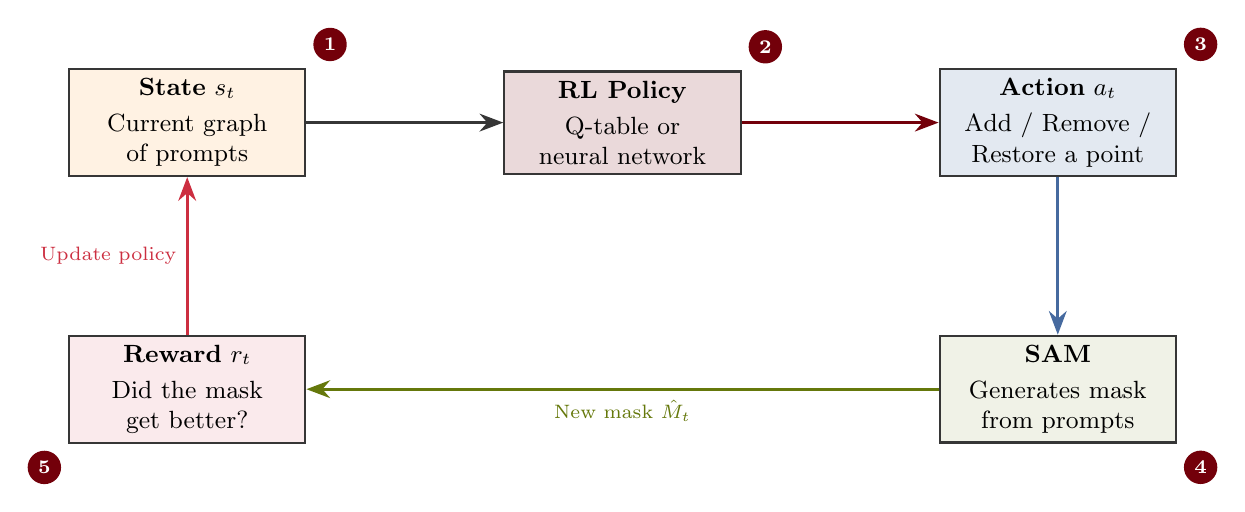
\begin{tikzpicture}[
    block/.style={draw=Black90, thick, minimum width=3.0cm, minimum height=1.2cm, align=center, font=\small},
    arr/.style={-{Stealth[length=3mm]}, very thick},
    every node/.style={font=\small}
]

% State
\node[block, fill=Sandstorm] (state) {
    \textbf{State} $s_t$\\[2pt]
    Current graph\\
    of prompts
};

% Policy
\node[block, fill=Garnet!15, right=2.5cm of state] (policy) {
    \textbf{RL Policy}\\[2pt]
    Q-table or\\
    neural network
};

% Action
\node[block, fill=Atlantic!15, right=2.5cm of policy] (action) {
    \textbf{Action} $a_t$\\[2pt]
    Add / Remove /\\
    Restore a point
};

% SAM
\node[block, fill=Horseshoe!10, below=2.0cm of action] (sam) {
    \textbf{SAM}\\[2pt]
    Generates mask\\
    from prompts
};

% Reward
\node[block, fill=Rose!10, below=2.0cm of state] (reward) {
    \textbf{Reward} $r_t$\\[2pt]
    Did the mask\\
    get better?
};

% Arrows
\draw[arr, Black90] (state) -- (policy);
\draw[arr, Garnet] (policy) -- (action);
\draw[arr, Atlantic] (action) -- (sam);
\draw[arr, Horseshoe] (sam) -- node[below, font=\scriptsize] {New mask $\hat{M}_t$} (reward);
\draw[arr, Rose] (reward) -- node[left, font=\scriptsize] {Update policy} (state);

% Step numbers
\node[circle, fill=Garnet, text=white, font=\scriptsize\bfseries, inner sep=2pt] at ($(state.north east)+(0.3,0.3)$) {1};
\node[circle, fill=Garnet, text=white, font=\scriptsize\bfseries, inner sep=2pt] at ($(policy.north east)+(0.3,0.3)$) {2};
\node[circle, fill=Garnet, text=white, font=\scriptsize\bfseries, inner sep=2pt] at ($(action.north east)+(0.3,0.3)$) {3};
\node[circle, fill=Garnet, text=white, font=\scriptsize\bfseries, inner sep=2pt] at ($(sam.south east)+(0.3,-0.3)$) {4};
\node[circle, fill=Garnet, text=white, font=\scriptsize\bfseries, inner sep=2pt] at ($(reward.south west)+(-0.3,-0.3)$) {5};

\end{tikzpicture}
\caption{\textbf{Step 3: The RL optimization loop.} \textcircled{1} The agent observes the current prompt graph. \textcircled{2} The policy decides what to do. \textcircled{3} It takes an action (add/remove/restore a point). \textcircled{4} SAM generates a mask using the updated prompts. \textcircled{5} The reward measures improvement and feeds back to the policy. This repeats for up to 100 steps per image.}
\label{fig:rl_loop}
\end{figure}


% ============================================================
% DIAGRAM 5: BEFORE AND AFTER OPTIMIZATION
% ============================================================
\section*{5. The Result: Better Prompts, Better Masks}

Over many iterations, the RL agent learns to remove unhelpful points and add informative ones, progressively improving the segmentation mask.

\begin{figure}[H]
\centering
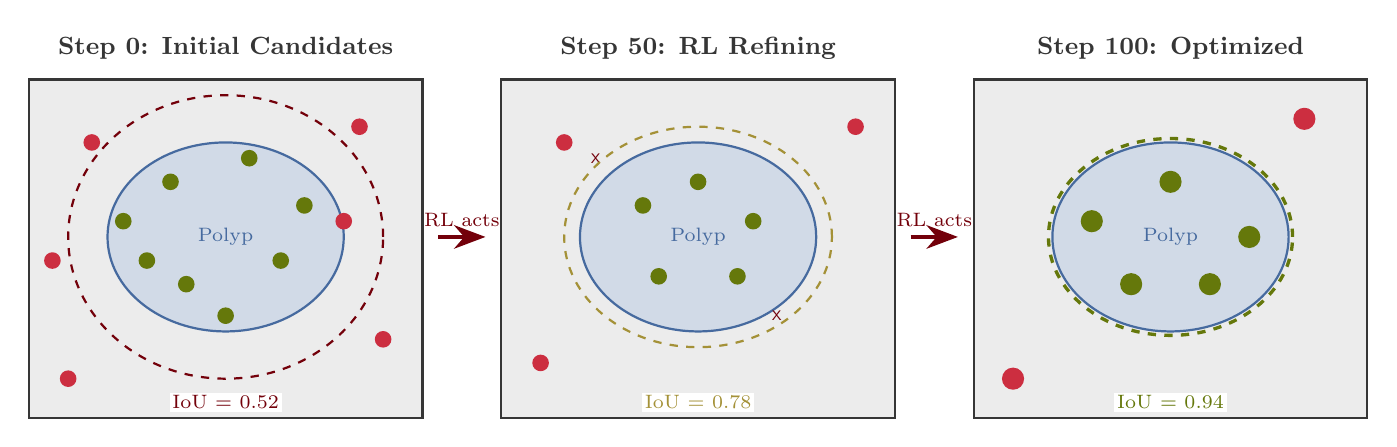
\begin{tikzpicture}[
    every node/.style={font=\small}
]

% === STEP 0: Initial (too many, messy) ===
\node[font=\small\bfseries, Black90] at (2.5, 5.2) {Step 0: Initial Candidates};
\draw[thick, Black90, fill=Black10] (0, 0.5) rectangle (5, 4.8);

% Polyp-like blob (medical image scenario)
\fill[Atlantic!25, draw=Atlantic, thick]
    (2.5, 2.8) circle [x radius=1.5, y radius=1.2];
\node[font=\scriptsize, Atlantic] at (2.5, 2.8) {Polyp};

% Many scattered points (messy)
\foreach \x/\y in {1.2/3.0, 1.8/3.5, 2.0/2.2, 2.8/3.8, 3.2/2.5, 3.5/3.2, 2.5/1.8, 1.5/2.5} {
    \fill[Horseshoe] (\x, \y) circle (3pt);
}
\foreach \x/\y in {0.5/1.0, 4.2/4.2, 0.8/4.0, 4.5/1.5, 0.3/2.5, 4.0/3.0} {
    \fill[Rose] (\x, \y) circle (3pt);
}

% Bad mask
\draw[Garnet, thick, dashed]
    (2.5, 2.8) circle [x radius=2.0, y radius=1.8];
\node[font=\scriptsize, Garnet, fill=white, inner sep=1pt] at (2.5, 0.7) {IoU = 0.52};


% === STEP 50: Getting better ===
\node[font=\small\bfseries, Black90] at (8.5, 5.2) {Step 50: RL Refining};
\draw[thick, Black90, fill=Black10] (6.0, 0.5) rectangle (11.0, 4.8);

% Same polyp
\fill[Atlantic!25, draw=Atlantic, thick]
    (8.5, 2.8) circle [x radius=1.5, y radius=1.2];
\node[font=\scriptsize, Atlantic] at (8.5, 2.8) {Polyp};

% Fewer, better-placed points
\foreach \x/\y in {7.8/3.2, 8.5/3.5, 9.2/3.0, 8.0/2.3, 9.0/2.3} {
    \fill[Horseshoe] (\x, \y) circle (3pt);
}
\foreach \x/\y in {6.5/1.2, 10.5/4.2, 6.8/4.0} {
    \fill[Rose] (\x, \y) circle (3pt);
}

% Removed points (X marks)
\foreach \x/\y in {7.2/3.8, 9.5/1.8} {
    \node[font=\tiny, Garnet] at (\x, \y) {\textsf{X}};
}

% Better mask
\draw[Honeycomb, thick, dashed]
    (8.5, 2.8) circle [x radius=1.7, y radius=1.4];
\node[font=\scriptsize, Honeycomb, fill=white, inner sep=1pt] at (8.5, 0.7) {IoU = 0.78};


% Arrow
\draw[-{Stealth[length=4mm]}, very thick, Garnet] (5.2, 2.8) -- node[above, font=\scriptsize] {RL acts} (5.8, 2.8);


% === STEP 100: Optimized ===
\node[font=\small\bfseries, Black90] at (14.5, 5.2) {Step 100: Optimized};
\draw[thick, Black90, fill=Black10] (12.0, 0.5) rectangle (17.0, 4.8);

% Same polyp
\fill[Atlantic!25, draw=Atlantic, thick]
    (14.5, 2.8) circle [x radius=1.5, y radius=1.2];
\node[font=\scriptsize, Atlantic] at (14.5, 2.8) {Polyp};

% Optimal points: spread across object, clean boundary
\fill[Horseshoe] (13.5, 3.0) circle (4pt);
\fill[Horseshoe] (14.5, 3.5) circle (4pt);
\fill[Horseshoe] (15.5, 2.8) circle (4pt);
\fill[Horseshoe] (14.0, 2.2) circle (4pt);
\fill[Horseshoe] (15.0, 2.2) circle (4pt);

% Tight negative boundary
\fill[Rose] (12.5, 1.0) circle (4pt);
\fill[Rose] (16.2, 4.3) circle (4pt);

% Excellent mask (nearly matches object)
\draw[Horseshoe, very thick, dashed]
    (14.5, 2.8) circle [x radius=1.55, y radius=1.25];
\node[font=\scriptsize, Horseshoe, fill=white, inner sep=1pt] at (14.5, 0.7) {IoU = 0.94};

% Arrow
\draw[-{Stealth[length=4mm]}, very thick, Garnet] (11.2, 2.8) -- node[above, font=\scriptsize] {RL acts} (11.8, 2.8);

\end{tikzpicture}
\caption{\textbf{Optimization over time.} The RL agent starts with many noisy candidate prompts (IoU = 0.52), iteratively removes bad ones and adds better ones (IoU = 0.78), and converges to a clean set of well-placed prompts that produce an accurate mask (IoU = 0.94). \textcolor{Horseshoe}{\textbf{+}} = foreground, \textcolor{Rose}{\textbf{--}} = background, \textcolor{Garnet}{\textsf{X}} = removed.}
\label{fig:optimization}
\end{figure}


% ============================================================
% DIAGRAM 6: OUR EXTENSIONS
% ============================================================
\section*{6. What We Propose to Change (Proposal 4 Extensions)}

The original system uses tabular Q-learning with a proxy reward. We propose four upgrades.

\begin{figure}[H]
\centering
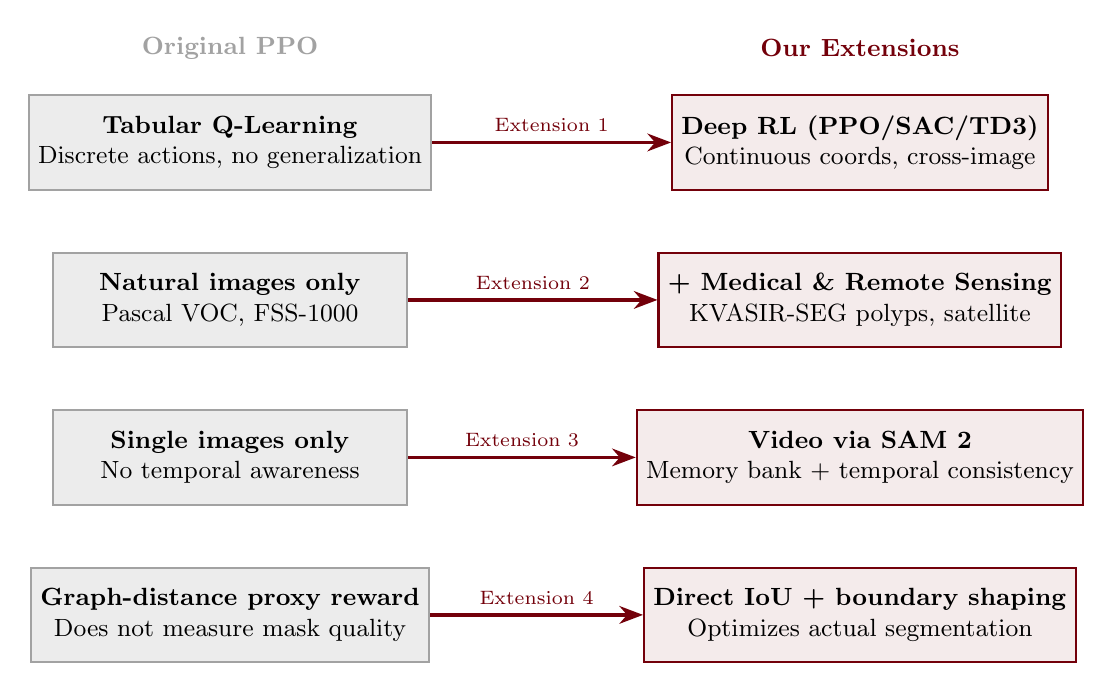
\begin{tikzpicture}[
    old/.style={draw=Black50, thick, fill=Black10, minimum width=4.5cm, minimum height=1.2cm, align=center, font=\small},
    new/.style={draw=Garnet, thick, fill=Garnet!8, minimum width=4.5cm, minimum height=1.2cm, align=center, font=\small},
    arr/.style={-{Stealth[length=3mm]}, very thick, Garnet},
    every node/.style={font=\small}
]

% Extension 1
\node[old] (old1) at (0, 5) {\textbf{Tabular Q-Learning}\\Discrete actions, no generalization};
\node[new] (new1) at (8, 5) {\textbf{Deep RL (PPO/SAC/TD3)}\\Continuous coords, cross-image};
\draw[arr] (old1) -- node[above, font=\scriptsize] {Extension 1} (new1);

% Extension 2
\node[old] (old2) at (0, 3) {\textbf{Natural images only}\\Pascal VOC, FSS-1000};
\node[new] (new2) at (8, 3) {\textbf{+ Medical \& Remote Sensing}\\KVASIR-SEG polyps, satellite};
\draw[arr] (old2) -- node[above, font=\scriptsize] {Extension 2} (new2);

% Extension 3
\node[old] (old3) at (0, 1) {\textbf{Single images only}\\No temporal awareness};
\node[new] (new3) at (8, 1) {\textbf{Video via SAM 2}\\Memory bank + temporal consistency};
\draw[arr] (old3) -- node[above, font=\scriptsize] {Extension 3} (new3);

% Extension 4
\node[old] (old4) at (0, -1) {\textbf{Graph-distance proxy reward}\\Does not measure mask quality};
\node[new] (new4) at (8, -1) {\textbf{Direct IoU + boundary shaping}\\Optimizes actual segmentation};
\draw[arr] (old4) -- node[above, font=\scriptsize] {Extension 4} (new4);

% Labels
\node[font=\small\bfseries, Black50] at (0, 6.2) {Original PPO};
\node[font=\small\bfseries, Garnet] at (8, 6.2) {Our Extensions};

\end{tikzpicture}
\caption{\textbf{Our four proposed extensions} to the Plug-and-Play PPO framework. Each replaces a limitation of the original system (left, gray) with an improved approach (right, garnet).}
\label{fig:extensions}
\end{figure}

\end{document}
